\subsection{Breakers}
\subsubsection{Breaker Overview}
The breaker system is half of the smart breakers system aimed at providing the consumer with better circuit protection in addition to circuit information. 

To achieve the goal of providing a system that is user friendly, the team decided to design smart breakers that the user can use in place of their current electro-mechanical breakers. This keeps installation simple and centralizes all parts of the system, making the system safer and more aesthetically pleasing.

\subsubsection{Breaker System Diagram}
\begin{figure}[htbp]
\begin{center}
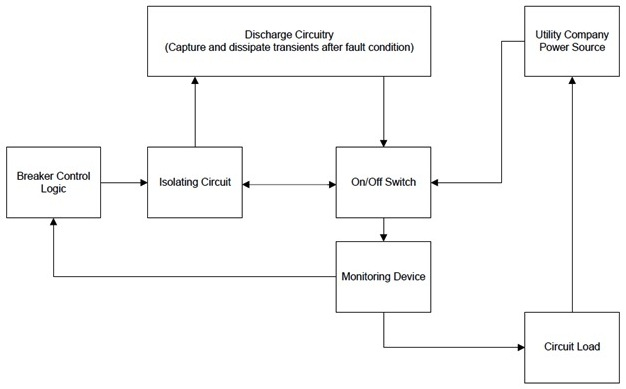
\includegraphics[width=6in]{includes/NJBreakerBlock}
\caption{Block diagram of breaker system}
\label{fig:breaker_block_diagram}
\end{center}
\end{figure}

The diagram above shows the breaker technology within the outlined box in relation to the other aspects of the smart breaker. The isolating circuit, the discharge circuitry and on/off switch are the three key components needed for a safe and fully functional breaker system.

\subsubsection{Component Selection}
On/Off Switch
The team focused initially on selecting an appropriate switching component and looked at SCRs, triacs, FETs, thyristors and solid state relays as possible options. The table below shows several benefits and drawbacks of each.

\begin{figure}[htbp]
\begin{center}
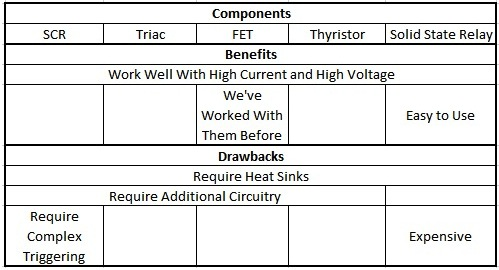
\includegraphics[width=5in]{includes/NJSwitchComponentOptions}
\caption{Table comparing switching components}
\label{fig:switch_component_options}  
\end{center}
\end{figure}

Ultimately, the team decided to use solid state relays, primarily due to their ease of use and lack of need for additional circuitry. This greatly reduced design time and allowed the team to focus on the primary goal of providing the user with power usage information. 

Isolation Circuit
The isolation circuitry's purpose is to protect the control logic should any line voltage cross over to the control side. The team selected an opto isolator for this purpose based on availability, ease of use, and functionality. 

Discharge Circuitry
At high currents and voltages, suddenly turning the circuit off can cause damaging transients. The discharge circuitry captures those transients before they become a problem and dissipates them later in a safe manner. For a final design, this component is important; however, it is not necessary to demonstrate the smart breakers' ability to read and control power and was not included in this prototype. 

\subsubsection{Testing}
Following selection of the switching component, the team ran a few basic tests and found that at low current levels the SSR provides as good or better functionality than standard air\-gap breakers. Turn on and turn off control voltages were also consistent, keeping the control logic simple.

\subsubsection{Future Work}
Solid state relays work well to demonstrate the smart breakers' ability to monitor and control electrical power, but are not a good selection for a consumer device because of high cost. Given more time, the team would like to design breakers that make use of another switching component at a lower cost and that minimize the need for heat sinks. Adding discharge circuitry is another aspect the team would like to include. 





